\textbf{3.1.} 三个点电荷分别位于边长为 $a$ 的正三角形的顶点，它们的电荷量分别为 $q, 2q$ 和 $-4q$ ，如图3.1所示. 试求这个系统的静电能(各电荷之间相互作用能的总和).

\vfill

\textbf{3.2.} 四个点电荷分别位于边长为 $a$ 的正方形的四个顶点，电荷量分别为 $q$ 和 $-q$ ，如图3.2所示.试求这个系统的静电能(各电荷之间相互作用能的总和).

\vfill

\newpage

\textbf{3.3.} 四个点电荷分别位于边长为 a 的正方形的四个顶点, 电荷量分别为 q 和 -q, 如图 3.3 所示. 试求这个系统的静电能(各电荷之间相互作用能的总和).

\vfill

\textbf{3.4.} 电荷量都是 q 的四个点电荷, 分别处在棱长为 a 的正四面体的四个顶点, 如图 3.4 所示. 试求这个系统的静电能(各电荷之间相互作用能的总和).

\vfill

\newpage

\textbf{3.5.} 正负离子相间排列成一条无穷长直线,相邻两离子间的距离都是 a, 已知正离子的电荷量为 q, 负离子的电荷量为 -q, 如图 3.5 所示. 试证明: 每个离子与所有其他离子间的相互作用能为 $W = -\frac{\ln 2}{2\pi \varepsilon_{0}} \frac{q^{2}}{a}$ .
\begin{center}
    
\includegraphics[width=0.5\linewidth]{figures/fig_3_5.jpg}
\end{center}

\vfill

\textbf{3.6.} 电偶极矩分别为 $p_1$ 和 $p_2$ 的两个电偶极子, 相距为 $r = |r|$ , $r$ 是从 $p_1$ 到 $p_2$ 的位矢, 如图3.6所示. 试证明: 当它们相距较远 (即 $r$ 比每个电


偶极子的线度都大很多)时,它们之间的相互作用能为

$$
W = \frac {r ^ {2} \boldsymbol {p} _ {1} \cdot \boldsymbol {p} _ {2} - 3 (\boldsymbol {p} _ {1} \cdot \boldsymbol {r}) (\boldsymbol {p} _ {2} \cdot \boldsymbol {r})}{4 \pi \varepsilon_ {0} r ^ {5}}
$$
\begin{center}
    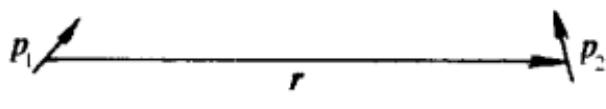
\includegraphics[width=0.5\linewidth]{figures/fig_3_6.jpg}
\end{center}

\vfill

\newpage

\textbf{3.7.} 电偶极矩分别为 $p_1$ 和 $p_2$ 的两个电偶极子，在同一平面内，相距为 $r, p_1$ 和 $p_2$ 与它们中心联线的夹角分别为 $\theta_1$ 和 $\theta_2$ ，如图3.7所示.试证明：它们之间的相互作用能为

$$
W = \frac {p _ {1} p _ {2}}{4 \pi \epsilon_ {0} r ^ {3}} (\sin \theta_ {1} \sin \theta_ {2} - 2 \cos \theta_ {1} \cos \theta_ {2})
$$

\vfill

\textbf{3.8.} 两个水分子相距为 $0.31\mathrm{nm}$ , 它们的电偶极矩大小相等, 都是 $6.2 \times 10^{-30}\mathrm{C} \cdot \mathrm{m}$ . 试求下列情况下它们之间的相互作用能: 它们的电偶极矩 (1) 都沿它们的联线且方向相同; (2) 一个沿它们的联线, 一个与联线垂直; (3) 两个都与它们的联线垂直且方向相同.

\vfill

\newpage

\textbf{3.9.} 当电荷连续分布时,求静电能量有三个公式

$$
W = \int u \mathrm{d} q\tag{I}
$$

$$
W = \frac {1}{2} \int U \mathrm{d} q\tag{Ⅱ}
$$

$$
W = \frac {1}{2} \iiint \boldsymbol {E} \cdot \boldsymbol {D} \mathrm{dV}\tag{Ⅲ}
$$

试分别说明这三个公式的物理意义,并以平行板电容器为例,分别用上列三个公式求它在电容为 C、蓄有电荷量 Q 时的静电能量.

\vfill

\textbf{3.10.} 空气中一半径为 $R$ 的导体球带有电荷量 $Q$ . (1) 试求它的静电能量 $W$ ; (2) 在半径为多大的球面内的电场能量为这能量的一半?

\vfill

\newpage

\textbf{3.11.} 空气中有一直径为 10cm 的导体球, 它的电势为 8000V, 试问它外面靠近表面处, 电场能量密度是多少?

\vfill

\textbf{3.12.} 电荷量 Q 均匀分布在半径为 R 的球体内, 试求它的静电能量.

\vfill

\newpage

\textbf{3.13.} 假定电子是球形的,并且它的静止能量 $mc^{2}$ (m 是它的静质量, c 是真空中光速) 就是来自它的静电能量. 这样就可以由它的电荷分布算出它的半径来. (1) 假定电子的电荷量 e 均匀分布在球面上, 试计算电子的半径; (2) 假定电子的电荷量 e 均匀分布在球体内, 试计算电子的半径; (3) 由于假定电荷分布情况不同, 算出的电子半径便稍有不同. 目前把 $r_{e} = \frac{1}{4\pi\varepsilon_{0}} \frac{e^{2}}{mc^{2}}$ 称为经典电子半径. 已知电子电荷的大小为 $e = 1.6 \times 10^{-19} C$ , 静质量为 $m = 9.1 \times 10^{-31} kg$ , 光速 $c = 3.0 \times 10^{8} m/s$ . 试计算 $r_{e}$ 的值.

\vfill

\textbf{3.14.} 设氢原子处在基态时, 核外电荷量的密度为 $\rho = -\frac{q}{\pi a^{3}} e^{-\frac{2r}{a}}$ , 式中 q 是电子电荷量的绝对值, a 是玻尔半径, r 是到核心的距离. 试求: (1) 这种电荷分布在氢核电场中的电势能; (2) 这种电荷分布本身的静电能量.

\vfill

\newpage

\textbf{3.15.} 导体上的电荷是这样分布的: 在达到静电平衡时, 使得电场的能量为最小(汤姆孙定理). 以一个有厚度的金属球壳为例, 当它带电时, 在电荷是球对称分布的情况下, 试论证: 只有电荷全都分布在外表面上, 电场的能量才是最小.

【论证】在电荷是球对称分布的情况下,根据对称性和高斯定理得球外的电场强度为

$$
E = \frac {Q}{4 \pi \varepsilon_ {0} r ^ {3}} r\tag{1}
$$

式中 Q 是球壳上的电荷量, $r = |r|$ , r 是自球心到场点的位矢. 于是得球外的电场能量为

$$
W _ {0} = \frac {\varepsilon_ {0}}{2} \iiint_ {V} E ^ {2} d V = \frac {\varepsilon_ {0}}{2} \int_ {R} ^ {\infty} \left(\frac {Q r}{4 \pi \varepsilon_ {0} r ^ {3}}\right) ^ {2} \cdot 4 \pi r ^ {2} d r = \frac {Q ^ {2}}{8 \pi \varepsilon_ {0} R}\tag{2}
$$

若电荷全都分布在外表面上，则外表面以内，电场强度处处为零，故这时电场的能量便为

$$
W = W _ {0}\tag{3}
$$

若电荷有一部分分布在外表面以内,如球壳体内或球壳的内表面上,则球壳体内的电场强度便不为零,设为 $E_{i}$ ,于是球壳体内的电场能量便为

$$
W _ {i} = \frac {\varepsilon_ {0}}{2} \iiint_ {V} E _ {i} ^ {2} \mathrm{d} V = \frac {\varepsilon_ {0}}{2} \int_ {0} ^ {R} E _ {i} ^ {2} \cdot 4 \pi r ^ {2} \mathrm{d} r = 2 \pi \varepsilon_ {0} \int_ {0} ^ {R} E _ {i} ^ {2} r ^ {2} \mathrm{d} r\tag{4}
$$

这时球壳外的电场不变,故球壳外的电场能量仍为 $W_{0}$ .于是电场的总能量便为

$$
\boldsymbol {W} = \boldsymbol {W} _ {0} + \boldsymbol {W} _ {i}\tag{5}
$$

因为

$$
W _ {i} = 2 \pi \epsilon_ {0} \int_ {0} ^ {R} E _ {i} ^ {2} r ^ {2} \mathrm{d} r \geqslant 0\tag{6}
$$

所以

$$
W \geqslant W _ {0}\tag{7}
$$

以上两式只有在 $E_{i} = 0$ 时才用等号. $E_{i} = 0$ 表明，外表面内无电荷，即电荷全都分布在外表面上.这时 $\pmb{W}$ 为最小，其值为 $W_{\mathrm{min}} = W_0$

\vfill

\textbf{3.16.} 一球形电容器由金属球和外面有厚度的同心金属球壳构成,充电后,两极分别带上等量异号电荷.设电荷都是球对称分布的,试论证:只有电荷全都分布在相向的两个表面上,电场的能量才是最小.

【论证】设球带电荷量 $Q$ ，壳带电荷量 $-Q$ .若 $Q$ 和 $-Q$ 分别球对称地分布在相向的两个表面上，则由对称性和高斯定理得，在离球心为 $r$ 处，电场强度为

$$
\pmb {E} _ {1} = 0, \quad r <   R _ {1} \text {或} r > R _ {2}\tag{1}
$$

$$
\boldsymbol {E} _ {2} = \frac {\boldsymbol {Q r}}{4 \pi \varepsilon_ {0} r ^ {3}}, \quad R _ {1} <   r <   R _ {2}\tag{2}
$$

式中 $R_{1}$ 是球的半径， $R_{2}$ 是壳的内半径， $r = |\boldsymbol{r}|$ ， $\boldsymbol{r}$ 是球心到场点的位矢。这时电场的能量为

$$
W _ {0} - \frac {\varepsilon_ {0}}{2} \iiint_ {V} E ^ {2} \mathrm{d} V = \frac {\varepsilon_ {0}}{2} \int_ {R _ {1}} ^ {R _ {2}} \left(\frac {Q r}{4 \pi \varepsilon_ {0} r ^ {3}}\right) ^ {2} \cdot 4 \pi r ^ {2} \mathrm{d} r = \frac {Q ^ {2}}{8 \pi \varepsilon_ {0}} \left(\frac {1}{R _ {1}} - \frac {1}{R _ {2}}\right)\tag{3}
$$

假定静电平衡时导体内有电荷分布, 如 Q 有一部分分布在球体内, -Q 有一部分分布在壳体内, 还有一部分分布在壳的外表面上, 则球与壳间的电场不变, 仍为式(2), 故球与壳间的电场能量仍然为式(3)中的 $W_{0}$ . 这时壳外的电场强度仍然为零. 但球体内和壳体内的电场强度便不为零. 设为 $E_{i}$ , 则因电场能量密度为

$$
w = \frac {1}{2} \boldsymbol {E} _ {i} \cdot \boldsymbol {D} _ {i} = \frac {\epsilon_ {0}}{2} E _ {i} ^ {2} \geqslant 0\tag{4}
$$

等号只在 $E_{i}=0$ 时用. 因此, 球体内和壳体内的电场能量为

$$
W _ {i} = \frac {\varepsilon_ {0}}{2} \iiint_ {V} E _ {i} ^ {2} d V \geqslant 0\tag{5}
$$

总的电场能量便为

$$
W = W _ {0} + W _ {i} \geqslant W _ {0}\tag{6}
$$

只有在球体内和壳体内均无电荷时,才能用等号.这个结果表明:在球对称分布的情况下,电荷只有全都分布在相向的两个表面上,电场的能量才是最小.

\vfill

\newpage

\textbf{3.17.} 一金属球外有一同心的、有厚度的金属球壳，球和壳原来都不带电，现将相同的电荷量 $Q$ 分别放在球上和壳上，设电荷都是球对称分布的。试问球上和壳上的电荷各如何分布，才使得电场能量为最小？

【解答】先考虑球上的电荷分布.因为是球对称分布,不论Q在球上如何分布,由对称性和高斯定理得出,Q在球外产生的电场强度都相同.只有Q全分布在球的表面上时,球内的电场强度才为零.这时球上电荷产生的电场能量为最小.

再考虑壳上的电荷分布,壳上的 Q 不论如何分布,只要是球对称分布,就不影响壳外的电场强度,且在壳的内表面以内产生的电场强度恒为零.由此可知,当壳体本身内的电场强度为零时,电场的能量便为最小.根据电荷守恒定律和高斯定理可知,这时壳的内表面上应分布着 Q,壳的外表面上应分布着 2Q.

总之，球上的 $Q$ 分布在表面上，壳上的 $Q$ 也分布在外表面上；同时，由于静电感应，壳的内表面上分布着 $-Q$ ，壳的外表面上又加上 $Q$ ，故分布着 $2Q$ 。这种分布所产生的电场能量为最小。

\vfill

\textbf{3.18.} 在电容率为 $\varepsilon$ 的无限大均匀介质中, 有一个半径为 R 的导体球带有电

荷量Q.试求电场的能量.

\vfill

\newpage

\textbf{3.19.} 半径为 2.0cm 的导体球外套有一个与它同心的导体球壳, 壳的内外半径分别为 4.0cm 和 5.0cm, 球与壳间以及壳外都是空气. 球和壳原来都不带电, 现在使球带电荷量 $3.0 \times 10^{-8}C$ , 试求这个系统的静电能量. 如果用导线把球与壳联在一起, 结果如何?

\vfill

\textbf{3.20.} 一球形电容器由半径分别为 $R_{1}$ 和 $R_{2}$ 的两个同心金属薄球壳构成，两壳间是空气。当它们带有等量异号电荷时，它们的电势差为 $U$ 。试求这电容器所储蓄的静电能量。

\vfill

\newpage

\textbf{3.21.} 电荷量 Q 均匀分布在一球壳体内, 壳体的内外半径分别为 a 和 b. 试求这个电荷系统的(1)电势能和(2)电场的能量.

\vfill

\textbf{3.22.} 电荷量 Q 均匀地分布在半径为 a 的球体内, 电荷量 - Q 均匀地分布在半径为 b 的同心球面上, 如图 3.22 所示. 试求这个系统的静电能量.

\vfill

\newpage

\textbf{3.23.} 在电容率为 $\varepsilon_{1}$ 的无限大均匀介质中，有一电容率为 $\varepsilon_{2}$ 、半径为 R 的均匀介质球，这球体内均匀地分布着电荷，其电荷量为 Q。试求静电能量。

\vfill

\textbf{3.24.} 一金属球外有一同心的金属球壳, 球和壳都带有电荷. 试论证, 用导线将球和壳联接起来, 这个系统的静电能量必定减少.

【论证】由于球上带有电荷,在球与壳联接之前,球与壳间有电场,壳外也有电场,这个系统的静电能量就等于这两处电场能量之和.由于电场能量密度 $w = \frac{1}{2} E \cdot D = \frac{\varepsilon}{2} E^2 > 0$ ,故两处电场能量均为正.用导线将球和壳联接后,球上电荷便全部跑到壳的外表面上去了.由于电荷都是球对称分布,所以球外的电场不变,因而电场的能量也不变.但球与壳间的电场消失了,因而电场能量为零.由于电场能量为正,故总的电场能量必定减少,所减少的值就等于原来球与壳间

的电场能量.

\vfill

\newpage

\textbf{3.25.} 半径为 $R$ 的一个雨点, 带有电荷量 $Q$ . 今将它打破成为两个完全相同的雨点并分开到相距很远. 试问静电能量改变多少?

\vfill

\textbf{3.26.} 铀 235 原子核可当作半径为 $R=9.2\times10^{-15}m$ 的球形, 它共有 92 个质子, 每个质子的电荷量为 $e=1.6\times10^{-19}C$ . 假定这些电荷量均匀分布在上述球体内. (1) 试求一个铀 235 原子核的静电能量; (2) 当一个铀 235 原子核分裂成两个相同的碎片, 每个都可当作均匀带电球体并相距很远时, 试求放出的能量; (3) 1kg 轴 235 裂变成上述碎片, 能放出多少能量?

\vfill

\newpage

\textbf{3.27.} 半径为 $a$ 的导体圆柱外套有一个内半径为 $b$ 的同轴导体圆筒, 它们的长度都是 $l$ , 圆柱与圆筒间充满电容率为 $\varepsilon$ 的均匀介质. 圆柱带有电荷量 $Q$ , 圆筒带有电荷量 $-Q$ . 略去边缘效应. (1) 试求圆柱与圆筒间离轴线为 $r$ 处的电场能量密度 $w$ ; (2) 试求整个介质内的电场能量 $W$ ; (3) 试证明: $W = \frac{1}{2} \frac{Q^2}{C}$ , 式中 $C$ 是圆柱和圆筒间的电容.

\vfill

\textbf{3.28.} 半径为 a 的长直导线外包有两层均匀介质, 内层介质的介电常数为$\varepsilon_{\mathrm{r1}}$ ，外半径为 $b$ ；外层介质的介电常数为 $\varepsilon_{\mathrm{r2}}$ ，外半径为 $c$ .试证明：当 $b^{(\varepsilon_{\mathrm{r1}} + \varepsilon_{\mathrm{r2}})} = a^{\varepsilon_{\mathrm{r2}}}$ $c^{\varepsilon_{\mathrm{r1}}}$ 时，若导线均匀带电，则两层介质内的电场能量相等.

\vfill

\newpage

\textbf{3.29.} 圆柱电容器由一长直导线和套在它外面的共轴导体圆筒构成,已知导线的半径为 a,圆筒的内半径为 b. 当这电容器蓄电时,略去边缘效应,试证明:这电容器所储存的能量有一半是在半径为 $r=\sqrt{ab}$ 的圆柱体内.

\vfill

\textbf{3.30.} 一厚为 $h$ 的无限大平板均匀带电, 电荷量密度为 $\rho$ . 今考虑这带电层内一个柱体, 它的轴线垂直于平板表面, 它的两底面则在板的两面上, 面积都是 $A$ . 试求这柱体内的电场能量.
\begin{center}
    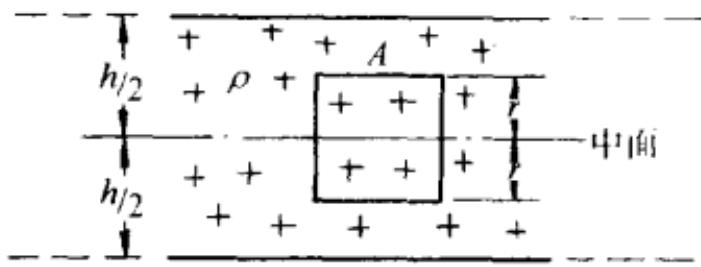
\includegraphics[width=0.5\linewidth]{figures/fig_3_30.jpg}
\end{center}

\vfill

\newpage

\textbf{3.31.} 一固体激光闪光灯的电源线路如图 3.31 所示, 其中电容 C 储存的能量, 通过放电, 为闪光灯提供能量. 已知 $C = 6000 \mu F$ , 球形开关间的击穿电压为 2000V. 试问: (1) 电容器在一次放电过程中, 能放出多少能量? (2) 若现有的电容器都是 $500 \mu F$ 、1000V 的, 要用几个这种电容器? 应如何联接?
\begin{center}
    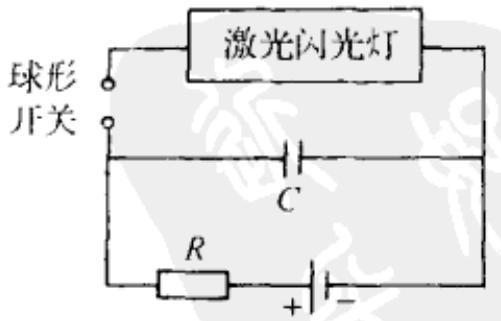
\includegraphics[width=0.5\linewidth]{figures/fig_3_31.jpg}
\end{center}

\vfill

\textbf{3.32.} 两个电容器的电容之比为 1:2, 将它们串联后接到电源上充电, 试问它们所储蓄的能量之比是多少? 如果将它们并联充电, 能量之比又是多少?

\vfill

\newpage

\textbf{3.33.} 两电容器的电容分别为 $C_1 = 10$ 皮法, $C_2 = 20$ 皮法. 将它们串联后充电到2.0伏. 试问它们各储蓄了多少能量?

\vfill

\textbf{3.34.} 两个相同的平行板电容器,极板都是半径为 $10\mathrm{cm}$ 的圆形,极板相距都是 $1.0\mathrm{mm}$ . 其中一个的两极板间是空气,另一个的两极板间是介电常数 $\varepsilon_{r} = 26$ 的酒精. 将这两个电容器并联后充电到 $120\mathrm{V}$ , 试求它们所储蓄的能量之和; 再断开电源, 将它们带异号电荷的两极板分别联在一起, 这时它们所储蓄的能量之和是多少?

\vfill

\newpage

\textbf{3.35.} 两电容器的电容分别为 $C_{1}$ 和 $C_{2}$ ，它们分别蓄有电荷量 $Q_{1}$ 和 $Q_{2}$ ，用导线联接如图 3.35(1) 所示。试证明：接通电键 K 后，它们所储蓄的电能将损失

$$
\frac {(C _ {2} Q _ {1} - C _ {1} Q _ {2}) ^ {2}}{2 C _ {1} C _ {2} (C _ {1} + C _ {2})}
$$
\begin{center}
    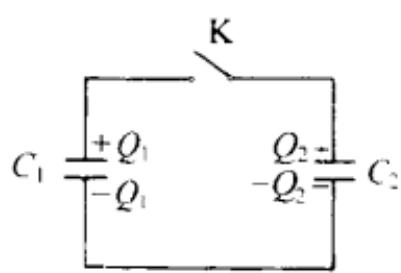
\includegraphics[width=0.5\linewidth]{figures/fig_3_35.jpg}
\end{center}

\vfill

\textbf{3.36.} 两平行金属板的面积都是 S，相距为 d，在它们中间平行地插入一块厚为 t、电容率为 $\varepsilon$ 的均匀介质片，如图 3.36 所示。略去边缘效应。试求下列两种情况下，插入介质片后静电能量变化的值：(1) 维持两板上的电荷量（一为 Q、一为 -Q）不变时插入介质片；(2) 维持两板的电势差 U 不变时插入介质片。
\begin{center}
    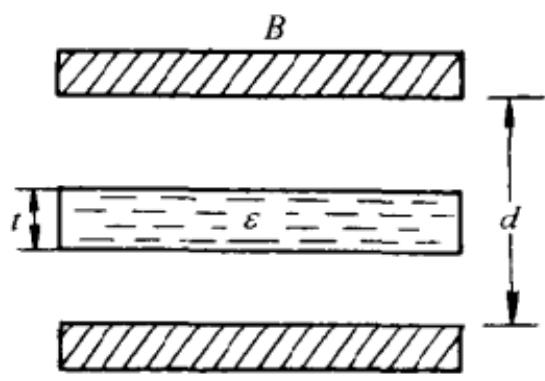
\includegraphics[width=0.5\linewidth]{figures/fig_3_36.jpg}
\end{center}

\vfill

\newpage

\textbf{3.37.} 一平行板电容器两极板的面积都是 S，其间充满了电容率为 $\varepsilon$ 的均匀介质，介质中的电场强度为 E。略去边缘效应。试证明：每个极板所受的静电力的大小为 $F = \frac{1}{2} \varepsilon E^{2} S$ 。

\vfill

\textbf{3.38.} (1)一空气平行板电容器两极板相距为 $1.0\mathrm{mm}$ , 加上 $1000\mathrm{V}$ 电压. 略去边缘效应, 试求极板单位面积上所受的静电力; (2)去掉电源, 再在两极板间充满介电常数为 $\varepsilon_{\mathrm{r}} = 2.0$ 的汽油, 极板单位面积上所受的静电力是多少? (3)如果先充汽油, 后加上 $1000\mathrm{V}$ 电压, 这时极板单位面积上所受的静电力又是多少?

\vfill

\newpage

\textbf{3.39.} 吸盘静电计(亦称开尔文静电计)是用来测量电势差的一种仪器,它由两块固定的平行金属板 A 和 B 构成,在上板中部挖出一块 C,C 可以上下活动,如图 3.39 所示.当上下板都不带电时,调整 C 使与 B 对齐,这时维持 C 的力为 $F_{1}$ ;当上下板都带电并有一定的电势差时,令 B

与 $C$ 的电势相同, 再调整 $C$ 使与 $B$ 对齐, 这时维持 $C$ 的力为 $F_{2}$ . 由两次维持 $C$ 的力之差 $F = F_{2} - F_{1}$ 和 $C$ 的面积 $S$ , 以及上下板之间的距离 $d$ , 便可以求出上下板的电势差 $U$ 来. (1) 试导出计算 $U$ 的公式 (以 $S, d, F$ 等表示); (2) 当 $S = 100 \mathrm{~cm}^{2}, d = 1.0 \mathrm{~mm}, F = 4.43 \times 10^{-4} \mathrm{~N}$ 时, 算出 $U$ 的值; (3) 试求灵敏度 $S = \frac{\mathrm{d} F}{\mathrm{d} U}$ 的值.

\vfill

\textbf{3.40.} 一静电伏特计由六对固定的和五对可转动的扇形金属片构成,相邻两片间的距离为 d，扇形角为 $90^{\circ}$ ，内半径为 $r_{1}$ ，外半径为 $r_{2}$ ，如图 3.40 所示。六对定片联接在一起成为一组，五对动片也联接在一起成为另一组。当定片与动片的电势差 U 保持不变，动片转到如图 3.40 所示的位置时，两组片同一边的夹角为 $\theta$ ，略去边缘效应，试求：(1) 这个系统储藏的静电能量 W；(2) 电场作用在动片上的力矩 M；(3) $r_{1} = 1.0 \, cm, r_{2} = 3.0 \, cm, d = 5.0 \, mm, U = 5.0$ 千伏时，M 的值。

(1) 主视图

(2)俯图视
\begin{center}
    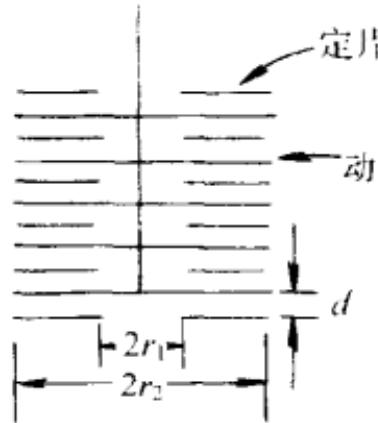
\includegraphics[width=0.5\linewidth]{figures/fig_3_40_1.jpg}
\end{center}
\begin{center}
    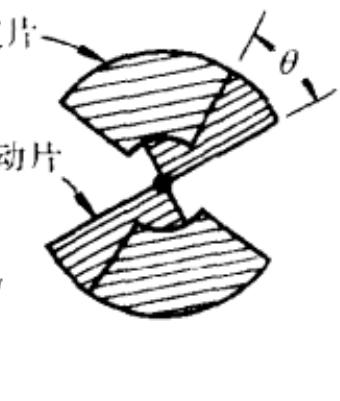
\includegraphics[width=0.5\linewidth]{figures/fig_3_40_2.jpg}
\end{center}

\vfill

\newpage

\textbf{3.41.} 一平行板电容器两极板的面积均为 $S$ ，极板间的距离为 $d$ 。将它充电到两极板的电势差为 $U$ 时，断开电源，然后把两极板分开到距离为 $2d$ 。略去边缘效应。试求：(1) 分开两极板所需的功；(2) 分开后两极板的电势差；(3) 分开后电容器所储存的能量。

\vfill

\textbf{3.42.} 一空气平行板电容器两极板的面积都是 $a \times b$ ，相距为 $d$ ，充电到电压为 $U$ 时断开电源，再将电容率为 $\varepsilon$ 的均匀介质充满两极板间。略去边缘效应。试求引入介质前后的静电能量之差，并证明这能量差等于电场力作的功。

\vfill

\newpage

\textbf{3.43.} 一空气平行板电容器两极板的面积都是 S，相距为 d，两板竖直放着，充电到电压为 U 时断开电源，再将它的下面一半浸入电容率为 $\varepsilon$ 的不导电的液体里。试问这电容器的静电能量减少了多少？减少的能量到哪里去了？（不考虑毛细现象和重力，并略去边缘效应。）

\vfill

\textbf{3.44.} 两平行金属板, 面积都是 $a \times b$ , 相距为 $d$ , 其间充满电容率为 $\varepsilon$ 的均匀介质, 两极板接到电压为 $U$ 的电池两极上; 现在将这介质沿平行于 $b$ 边抽出一段, 如图3.44所示. 略去边缘效应, 试求电场把介质拉回去的力.

\vfill

\newpage

\textbf{3.45.} 一平行板电容器的两极板都是面积为 $a \times b$ 的长方形金属片, 相距为 $d$ , 分别带有电荷量 $Q$ 和 $-Q$ . 一块厚为 $t$ , 介电常数为 $\varepsilon_{r}$ 的均匀介质片, 其面积与极板相同, 平行地放在电极板间. 今将这介质片从两极板间沿长度方向平行地抽出, 当还有长为 $x$ 的一段尚在两极板间时, 如图 3.45 所示. 略去边缘效应, 试求电场作用在介质片上的力.
\begin{center}
    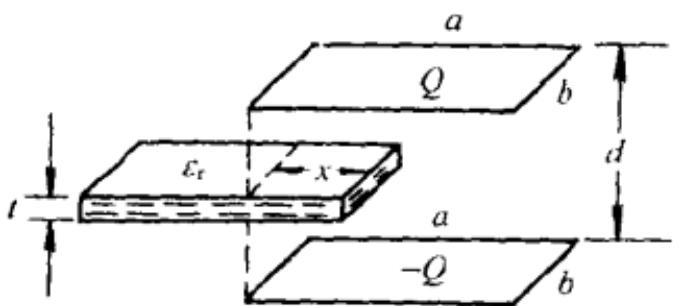
\includegraphics[width=0.5\linewidth]{figures/fig_3_45.jpg}
\end{center}

\vfill

\textbf{3.46.} 一平行板电容器两极板的面积都是 S，相距为 d，其间有一块厚为 t、介电常数为 $\varepsilon_{r}$ 的平行介质平板，如图 3.46 所示，接通电键 K，使这电容器充电到电压为 U。略去边缘效应。（1）断开电源，把介质板抽出，试问需要作多少功？（2）如果在不断开电源的情况下抽出介质板，则要作多少功？

\vfill

\newpage

\textbf{3.47.} 一平行板电容器两极板的面积都是 S，相距为 d，其间有一块厚为 t 的平行导体片，如图 3.47 所示，接通电键 K，使这电容器充电到电压为 U。略去边缘效应。（1）断开电源，把导体片抽出，试问需要作多少功？（2）如果在不断开电源的情况下抽出导体片，则要作多少功？
\begin{center}
    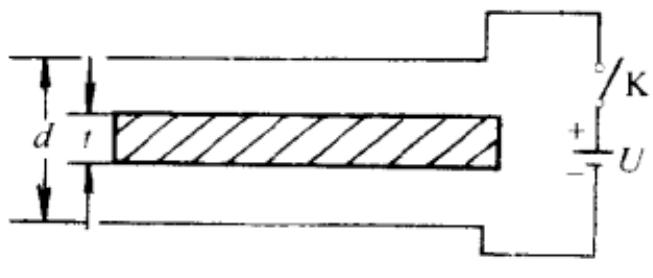
\includegraphics[width=0.5\linewidth]{figures/fig_3_47.jpg}
\end{center}

\vfill
